\section{Evaluation of the ABSNF} \label{sec_evaluation}
\subsection{Problem Specification}
Given is a PL function in abs-normal form. The evaluation of it means calculating the vectors $\Delta y$ and $\Delta z$:
\begin{flalign}
\Delta y &= b + (J \times \Delta x) + (Y \times |\Delta z|) \label{eval_1}\\
\Delta z &= a + (Z \times \Delta x) + (L \times |\Delta z|) \label{eval_2}
\end{flalign}
where the following structures are given:
\begin{flalign*}
a,b,Z,L,J,Y,m,n,s, \Delta x
\end{flalign*}
In (\ref{eval_2}) $\Delta z$ depends on the element-wise absolute function of its own and therefore it cannot be calculated with a simple matrix vector dot product. The matrix $L$ is lower triangular and therefore the vector $\Delta z$ can be iteratively calculated, by taking the row-wise dot product of $L$ and $|\Delta z|$. \\

To illustrate the process, consider:
\begin{flalign*}
k = a + Z \times \Delta x
\end{flalign*}

Now we calculate $\Delta z$ element-wise:

\begin{flalign*}
\highlightblue{\Delta  z_1}  &= \underbrace{L_1 \times |\Delta z|}_{=0} + k_1 = k_1 \\
\highlightyellow{\Delta z_2} &= L_2 \times |\Delta z| + k_2 \\
	&= L_{2,1} \times \highlightblue{|\Delta z_1 |} + k_2 \\
\highlightgreen{\Delta z_3} &= L_3 \times |\Delta z| + k_3 \\
	&= L_{3,1} \times \highlightblue{|\Delta z_1 |} + L_{3,2} \times \highlightyellow{|\Delta z_2|} + k_3 \\
\highlightred{\Delta z_4} &= L_{4} \times |\Delta z| + k_4 \\
	&= L_{4,1} \times \highlightblue{|\Delta z_1|} + 
	L_{4,2} \times \highlightyellow{|\Delta z_2|} +
	L_{4,3} \times \highlightgreen{|\Delta z_3|} + k_4 \\
	....
\end{flalign*}

\subsection{Implementation}
Our implementation is focused on speed and  demands the device to hold all the required data structures in global memory simultaneously. \\
Given this premise, the calculation of (\ref{eval_1}) and (\ref{eval_2}) is a series of dot products and therefore is highly parallelize-able. For this we relied mainly on CUBLAS routines. 
A simplified version of our implementation can be found in fig. \ref{fig_lst_eval}.

\begin{figure}
\begin{lstlisting}[language=cpp]
template <typename T>
void eval(T *a, T *b, T *Z, T *L, T *J, T *Y, T *dx,
		  int m, int n, int s, T *dz, T *dy, T *abs_dz)
{
	// dz = a
	cudaMemcpy(dz, a, ., cudaMemcpyDeviceToDevice));
	// dz = Z * dx + dx
	cublasDgemv(.,Z, ., dx, . dz, .)
	// dz[i] = L[i]_i * |dz|_i
	for(int i=0; i<s; i++)
	{
		cublasDgemv( . ,&L[i * s], . ,abs_dz, . , &dz[i],.);
		abs <<<1,1>>>(&dz[i], &abs_dz[i], 1);
	}
	// dy = b
	cudaMemcpy(dy, b, ., cudaMemcpyDeviceToDevice);
	// dy = dy + J*dx
	cublasDgemv(.,J, ., dx, ., dy, .));
	// dy = dy + Y * |dz|
	cublasDgemv(., Y, ., abs_dz, ., dy, .));
}
\end{lstlisting}
\caption{Simplified version of the evaluation implementation \label{fig_lst_eval}}
\end{figure}

\subsection{Performance Experiments}
For our experiments and the subsequent analysis, we equalized the dimensions of given data-structures:
\begin{flalign*}
	m = n = s
\end{flalign*}

\subsubsection{Single Execution of the evaluation function}

In this experiment, we executed the serial python- as well as the parallel CUDA implementations for different dimensions of $s$ and measured the runtime (fig. \ref{eval_single_repetition}). Since the results were not as expected in favor of the CUDA implementation, we also dismantled the runtime on the parallel devices and measured the "data-upload-time" and the "execution-only-time" separately (fig. \ref{eval_memory}).

\begin{figure}[ht]
	\centering
	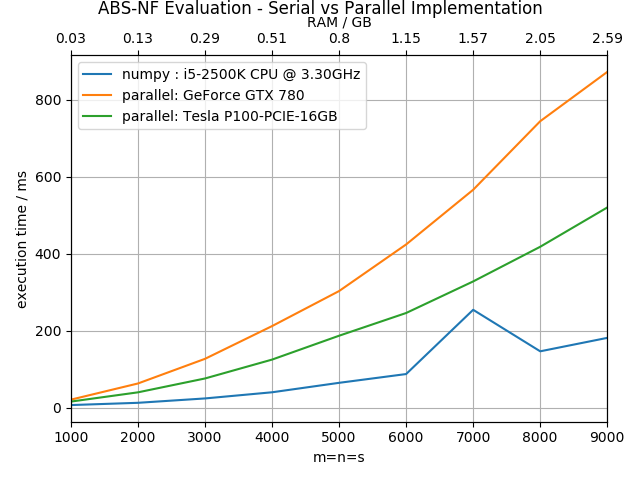
\includegraphics[width=0.7\textwidth]{img/eval_single_repetition.png}
	\caption{Single execution of the evaluation function on different devices.}
	\label{eval_single_repetition}
\end{figure}

\begin{figure}[ht]
	\centering
	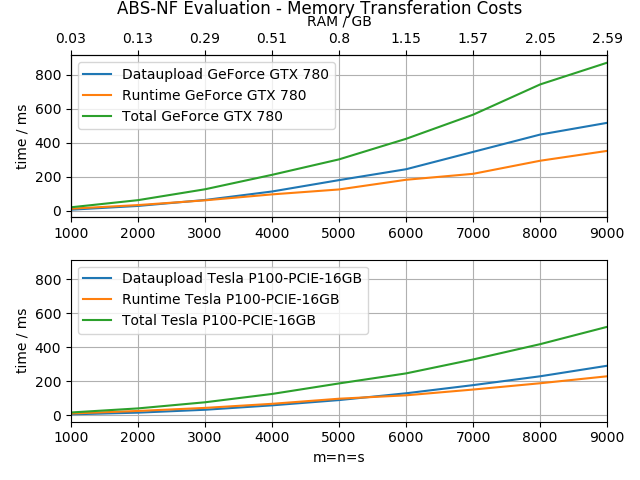
\includegraphics[width=0.7\textwidth]{img/eval_memory.png}
	\caption{Data-transfer and execution time of the parallel implementation}
	\label{eval_memory}
\end{figure}

\subsubsection{Multiple Executions of the evaluation function}

Since the scenario of evaluating the function just once is not quite realistic, we did a second experiment, where we uploaded data onto the devices and executed the evaluation routine a 1000 times. Here we only measured the pure execution time without the data-transfer, since the upload time should be marginal with a high enough number of executions. The results can be found in fig. \ref{eval_1000}.

\begin{figure}[ht]
	\centering
	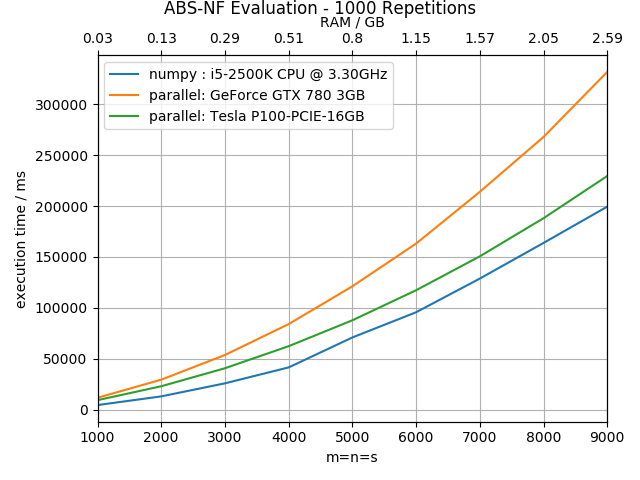
\includegraphics[width=0.7\textwidth]{img/eval_mult_repetition.png}
	\caption{Multiple executions of the evaluation function on different devices}
	\label{eval_1000}
\end{figure}

\subsubsection{Experiment Analysis}

Here we can clearly see, that the transfer time, which is the time that it takes to upload the required data structures onto the device is extremely significant and takes a disproportional high share of the total time.

The results of the experiment are heavy in favor of the serial implementation.\\
For data, that completely fits into the global memory of the device, we couldn't measure any performance gains through the CUDA implementation on given devices (fig \ref{eval_single_repetition} and  fig. \ref{eval_1000}). The simplistic and serial numpy version even outperforms the cuda version running on the tesla device.

If the data structures get that big, such that they don't fit into the global memory of the device, we can expect the parallel versions' performance to be even worse, since the data-transfer time takes a disproportional high share of the overall runtime (fig. \ref{eval_memory}).

The complexity of the evaluation function is $O(s^2)$. The memory also grows quadratic depending on the variable $s$ and therefore we get a memory complexity of $O(s^2)$, which may explain the bad results of the experiment.

We therefore come to the conclusion, that the considerable effort of implementing a parallel version of the evaluation function is not worth the effort.

